\subsection{UI Design}\label{sec:ui-design}

When designing the UI of Notipie,
I tried to maximize usability,
and minimize complexity of the interface.

Maintaining simplicity of the interface is not an easy task,
so I took inspiration from the professional designs.

\subsubsection{Inspirations}\label{sec:inspirations}

My main inspirations for the interface were
Apple Human Interface Guidelines~\cite{apple_inc_human_2022}
and Google's Material Design~\cite{google_llc_material_2022},
but by far the most inspiration was taken from
Github Primer~\cite{github_inc_primer_2022}.

I tried to break down what is useful,
what is unnecessary in my project,
and extract only the essentials for my design.

Adam Wathan and Steve Schoger
also had a great influence
on my design decisions.
Their book,
\citetitle{wathan_refactoring_2018}~\cite{wathan_refactoring_2018}
was an excellent guidance of the best practices
of the modern user interface design.

\subsubsection{Final design}\label{sec:final-design}

\paragraph*{The card}\label{par:the-card}

The card is a building block for the entire user interface.
It provides the most interaction in the whole application,
therefore it had to be designed with clearly laid out information
and intuitive controls.

\begin{figure}[h]
      \centering
      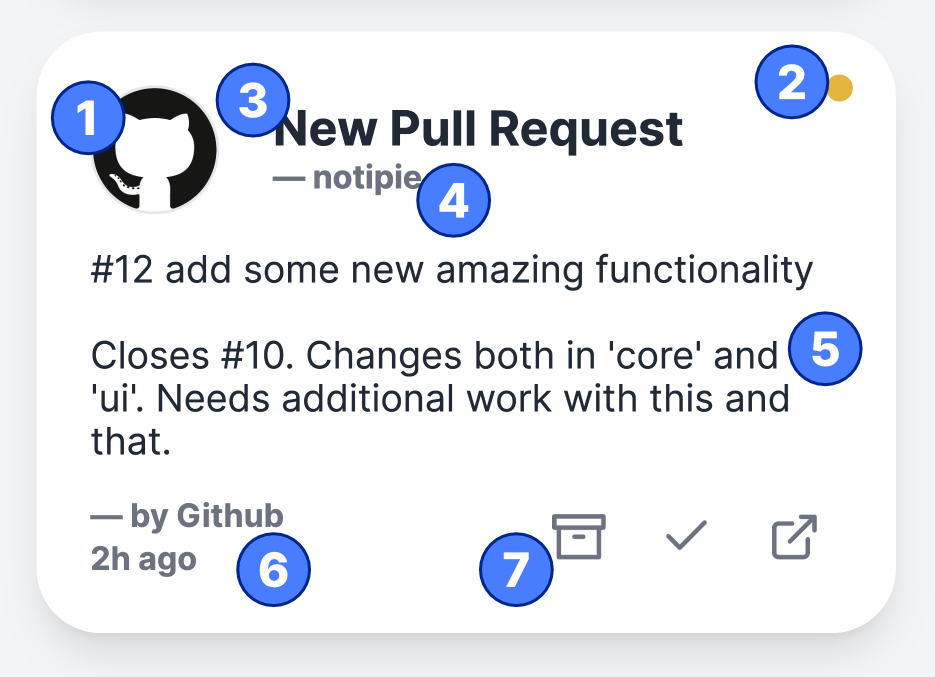
\includegraphics[width=8cm,keepaspectratio]{img/card_labeled.png}
      \caption{The card with labeled elements}
      \label{fig:card-with-labeled-elements}
\end{figure}

The card itself consists of several elements,
as depicted in figure~\ref{fig:card-with-labeled-elements}:

\begin{enumerate}
      \item
            logo,
            it can be an image
            or automatically generated SVG
            from the first two letters of the app's name,
      \item
            indicator,
            whether the notification has been seen or not,
      \item
            title of the notification,
      \item
            subtitle,
      \item
            body,
            that collapses after it reaches a certain length,
            so that an ellipsis appears (\texttt{...}),
      \item
            information about what app sent the notification and when it happened,
      \item
            controls to archive,
            mark as read,
            or go to external site connected with the notification,
            like a certain build on Jenkins,
            or the notification page on Github.
\end{enumerate}

\begin{figure}[h]
      \centering
      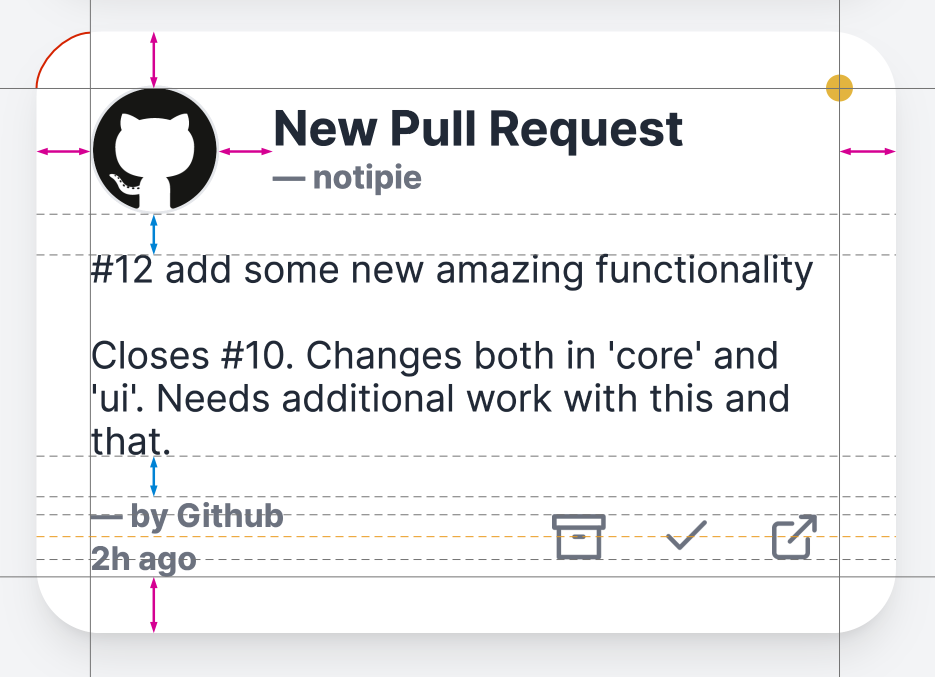
\includegraphics[width=8cm,keepaspectratio]{img/card_guides.png}
      \caption{The card with guides}
      \label{fig:card-with-guides}
\end{figure}

The card was also designed with aesthetics in mind.
All elements were carefully positioned and aligned,
so they are not only pleasant to look at,
but also have features important for visual communication.

Those features, highlighted in figure~\ref{fig:card-with-guides}, include:

\begin{itemize}
      \item
            the rounded corners take the focus away from the card frame,
            and provide a natural, neutral enclosure for the notification,
      \item
            the inner padding is of equal size in each direction
            to provide optical stability,
      \item
            the distance between the logo and title -- subtitle combo
            is the same size as the padding,
            making the logo appear centered,
      \item
            the title -- subtitle combo itself
            is centered vertically relative to the logo,
      \item
            the distances between the logo,
            notification body, and app name -- timestamp combo are shorter
            in order to make the inner section more connected,
      \item
            the controls are centered relative to the app name -- timestamp combo,
      \item
            the \textit{unread} indicator is unobtrusive enough
            not to steal all the focus from the card's content,
      \item
            finally, the \textit{unread} indicator
            is positioned slightly outside the inner section,
            so that it belongs to the card itself,
            not its content,
            therefore it is easier to spot at a glance.
\end{itemize}
